\documentclass[mathserif,18pt,xcolor=table]{beamer}

\usepackage {bbm}
\usepackage {textpos}
\usepackage{tikz}
\usepackage{graphicx}
\usepackage{calc}
\graphicspath{{figures/}}


\definecolor{tamumaroon}{RGB}{80,0,0}
\definecolor{tamublack}{RGB}{51,44,44}
\definecolor{tamugray}{RGB}{143,143,140}
\definecolor{tamumustard}{RGB}{244,175,0}
\definecolor{tamugreen}{RGB}{126,122,0}
\definecolor{tamuolive}{RGB}{79,85,42}


\mode<presentation>
{
% \usetheme{Pittsburgh}
\usetheme{Boadilla}
\usefonttheme[onlymath]{serif}

% Exclude Default Navigation tools
\setbeamercovered{invisible}
\setbeamertemplate{navigation symbols}{}

% Color Theme
\setbeamercolor{normal text}{bg=white,fg=tamublack}
\setbeamercolor{structure}{fg=tamumaroon}
\setbeamercolor{alerted text}{fg=red!85!black}
\setbeamercolor{item projected}{use=item,fg=black,bg=item.fg!35}
\setbeamercolor*{palette primary}{use=structure,fg=white, bg=tamumaroon}
\setbeamercolor*{palette secondary}{use=structure,bg=tamugray}
\setbeamercolor*{palette tertiary}{use=structure,bg=tamugreen}
\setbeamercolor*{palette quaternary}{use=structure,fg=structure.fg,bg=tamumustard}
% \setbeamercolor*{frametitle}{use=structure,fg=utorange, bg=utsecbrown}
\setbeamercolor*{framesubtitle}{fg=tamublack}
\setbeamercolor*{block title}{parent=structure,fg=black,bg=tamuolive}
\setbeamercolor*{block body}{fg=black,bg=tamublack!10}
\setbeamercolor*{block title alerted}{parent=alerted text,bg=black!15}
\setbeamercolor*{block title example}{parent=example text,bg=black!15}

\setbeamerfont{framesubtitle}{size=\normalsize}
}

%% For widescreen format
% \usepackage[orientation=landscape,size=custom,width=16,height=9,scale=0.5,debug]{beamerposter}

%% Make Footer Designs
\makeatletter
\setbeamertemplate{footline}
{
\leavevmode%
\hbox{%
\begin{beamercolorbox}[wd=.333333\paperwidth,ht=2.25ex,dp=1ex,center]{author in head/foot}%
  \usebeamerfont{author in head/foot}\insertshortauthor%~~\beamer@ifempty{\insertshortinstitute}{}{(\insertshortinstitute)}
  \end{beamercolorbox}%
  \begin{beamercolorbox}[wd=.333333\paperwidth,ht=2.25ex,dp=1ex,center]{title in head/foot}%
    \usebeamerfont{title in head/foot}\insertshorttitle
    \end{beamercolorbox}%
    \begin{beamercolorbox}[wd=.333333\paperwidth,ht=2.25ex,dp=1ex,right]{date in head/foot}%
      \usebeamerfont{date in head/foot}\insertshortdate{}\hspace*{2em}
      \insertframenumber{} / \inserttotalframenumber\hspace*{2ex}
      \end{beamercolorbox}}%
      \vskip0pt%
      }
      \makeatother

      \usepackage{kerkis}
      \usepackage[T1]{fontenc}
      \usepackage[protrusion=true,expansion=true]{microtype}
      \usepackage{amsmath}
      \usepackage{graphicx}


      \renewcommand*{\thefootnote}{\fnsymbol{footnote}}


      \pgfdeclareimage[height=2.0cm]{tamuecenbig}{figures/ecen_stacked}
      \pgfdeclareimage[height=0.6cm]{tamu}{figures/TAM-Wordmark}
      \pgfdeclareimage[height=1.5cm]{tamustack}{figures/TAM-Stack}
      % \pgfdeclareimage[height=1.0cm]{scsmall}{logos/SC12}

      \title{Sommerfeld Integral}
      \subtitle{Horizontally Oriented Magnetic Dipole above Silver Half-plane}
      \author[Hasan Tahir Abbas]{ \underline{Hasan~Tahir~Abbas}}

      \institute{Department of Electrical  \& Computer Engineering\\ \mbox{} \\ \pgfuseimage{tamuecenbig}}
      \date[Spring 2016]{}

      \begin{document}

      \tikzstyle{block} = [rectangle, draw, rounded corners, shade, top color=white, text width=5em,
      bottom color=blue!50!black!20, draw=blue!40!black!60, very thick, text centered, minimum height=4em]
      \tikzstyle{line} = [draw, -latex']
      \tikzstyle{cloud} = [draw, ellipse,top color=white, bottom color=red!20, node distance=2cm, minimum height=2em]


      \beamertemplateballitem
      %\beamertemplatetransparentcoveredhigh

      \frame{\titlepage}

      % \addtobeamertemplate{frametitle}{}{%
      % \begin{tikzpicture}[remember picture,overlay]
      % \node[anchor=north east,yshift=0pt] at (current page.north east) {
\includegraphics[scale=1]{TAM-Wordmark}};
      % \end{tikzpicture}
      % }
      % Add TAMU logo on each slide in the north-east side
      % Shifted to be right at the edge
      \addtobeamertemplate{frametitle}{}{%
      \begin{tikzpicture}[remember picture,overlay]
        \node[anchor=north east,yshift=5pt,xshift=2pt] at (current page.north east) {
\includegraphics[height=.7cm]{ecen}};
      \end{tikzpicture}}

      \section{Plasma waves in the Terahertz frequency}
      % ------------------------------------------------------------
      % ------------------------------------------------------------
      % ------------------------------------------------------------
      % ------------------------------------------------------------
      % ------------------------------------------------------------
      % ------------------------------------------------------------
      % ------------------------------------------------------------
      \begin{frame}
        \frametitle{Integration Contour}
        \framesubtitle{haha}  %% needed for proper positioning of the logo ...
        \begin{columns} % align columns
          \begin{column}{.5\textwidth}
            For 3D structures
            \begin{equation} \label{N_3d}
              \omega _{p,3D} = \sqrt {\dfrac {e^{2}N_{3D}} {\varepsilon \varepsilon _{0}m^{\ast }}}
            \end{equation}
            % \includegraphics[scale=0.220]{dispersion_3d.pdf}
            \end{column}%
            \hfill%

            \begin{column}{.5\textwidth}
              For 2D sheet based structures
              \begin{equation} \label{N_2d}
                \omega_{p,2D}=\sqrt {\dfrac {e^{2}N_{2D}} {2\varepsilon \varepsilon _{0}m^{\ast }}k}
              \end{equation}
              % \includegraphics[scale=0.220]{dispersion_2d.pdf}
              \end{column}%
            \end{columns}
          \end{frame}
          % ------------------------------------------------------------
          % ------------------------------------------------------------
          % ------------------------------------------------------------
          % ------------------------------------------------------------
          % ------------------------------------------------------------
          % ------------------------------------------------------------
          % ------------------------------------------------------------
          \section{Surface Plasmons in the Terahertz frequency regime}
          \begin{frame}
            \frametitle{Two-dimensional Electon Gas (2DEG)}
            \framesubtitle{Introduction}
            \begin{columns} % align columns
              \begin{column}{.5\textwidth}
                \begin{minipage}[c][.6\textheight][c]{\linewidth}
                  \begin{itemize}
                    \item Semiconductor Interface
                    \item Quantum Well
                    \item High electron Mobility
                    \item High Charge concentration
                  \end{itemize}
                \end{minipage}
              \end{column}

              \begin{column}{.5\textwidth}
                % 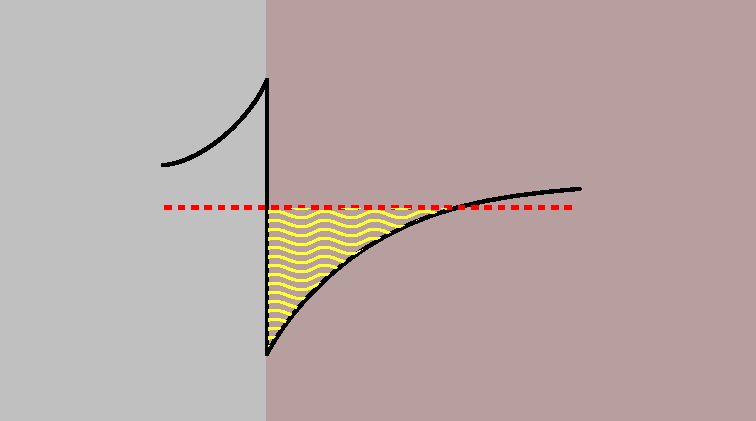
\includegraphics[width=\linewidth,keepaspectratio]{figures/2deg_bandgap.pdf}

                % Use this to preserve fonts from Inkspace
                \begin{figure}
                  \def\svgwidth{\linewidth}
                  \input{figures/2deg_bandgap.pdf_tex}
                \end{figure}
                \end{column}%
              \end{columns}
            \end{frame}
              % ------------------------------------------------------------
              % ------------------------------------------------------------
              % ------------------------------------------------------------
              % ------------------------------------------------------------
              % ------------------------------------------------------------
              % ------------------------------------------------------------
              % ------------------------------------------------------------
              \end{document}
